%-----------------------------------------------------------
%   Capítulo 5 - Arquitectura e Projecto do Sistema
%-----------------------------------------------------------
\chapter{Projecto}
Neste capitulo será abordado o \textit{hardware} e \textit{software} a ser aplicado para o projeto final.

\section{Arquitectura do Sistema}

A arquitectura do projeto tem por base um \textit{master} que recebe por \textit{Controller Area Network} (CAN) os valores em lux dos vários \textit{slaves}, para calcular os valores do \textit{roll}, \textit{pitch} e \textit{yaw} do sistema.

\begin{figure}[!htb]
\centering
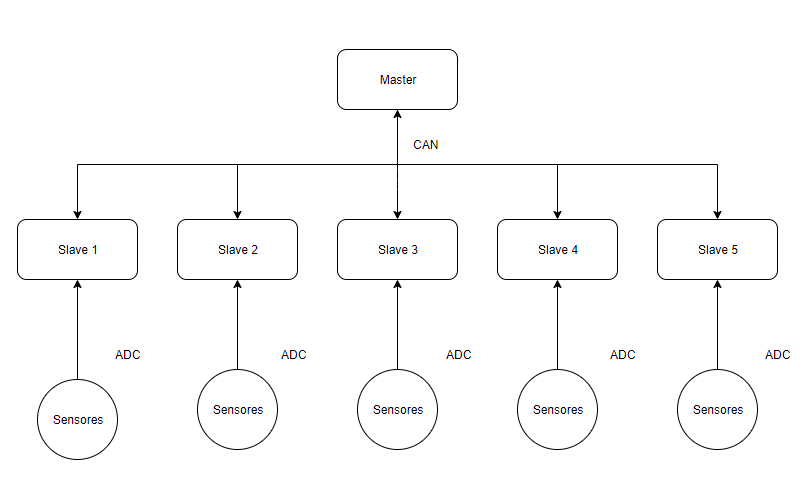
\includegraphics[scale=0.65]{Figuras/alto_n.PNG}
\caption{Arquitectura de alto nível do projeto como um todo}
\label{Rotulo}
\end{figure}

\section{Protocolo de comunicação implementado}

O protocolo implementado consiste no \textit{master} enviar o ID do \textit{slave} e o \textit{slave} responder com o valor do \textit{roll} e o maior valor em lux do anel, ou caso o master envie o ID 0x10, o anel é calibrado, para que a posição que  se está a obter o valor em lux mais alto passe a ser os 0º.

\section{Descrição de \textit{Hardware}}

\begin{itemize}
        \item STM32 F103RB;
        \item 8 díodos;
        \item 8 resistências 2.2k$\Omega$;
        \item 1 CAN \teztit{Transceiver} VP230.
\end{itemize}

\subsection{STM32F103RB}
O STM32F103RB é um sistema embebido que incorpora um ARM Cortex-M3, memórias embebidas de alta velocidade e uma ampla variedade I/Os. É composto por 12-bits ADC, bem como várias interfaces de comunicação: dois I2Cs e SPIs, 3 USARTs, USB e CAN. 

\subsection{Resistência dependente da luz (LDR)}
O LDR é uma resistência dependente da luz, quanto maior for a incidência de luz no componente menor será a sua resistência e vice-versa.
O LDR é constituído por um material semicondutor com elevada resistência.
Quando a luz incide sobre o LDR este tende a libertar electrões que irão melhorar a sua condutividade.

\begin{figure}[!htb]
\centering
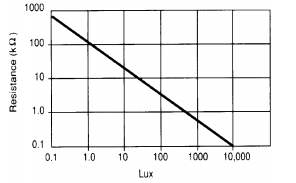
\includegraphics[scale=1]{Figuras/ldr.PNG}
\caption{Resistência em função da luminosidade}
\label{Rotulo}
\end{figure}

\subsection{CAN \teztit{Transceiver} VP230}

De um modo geral, um CAN \textit{Transceiver} um componente usado para arbitrar o envio e recepção de mensagens CAN no barramento físico. Ou seja, é algo que converte a mensagem para algo que seja possível enviar para o barramento e faz o contrário em que "traduz" o sinal do barramento para algo que o \textit{software} do micro-controlador possa ler. 



\section{Descrição do \textit{Software}}

Em termos da arquitetura de \textit{software} implementada no \textit{slave}, consiste em realizar todas as inicializações necessárias para o \textit{analog-to-digital converter} (ADC) e CAN, em seguida os dados dos sensores são lidos e convertidos para Lux, e por fim é verificado se o \textit{slave} em questão é requisitado para o envio dos dados.

\begin{figure}[!htb]
\centering
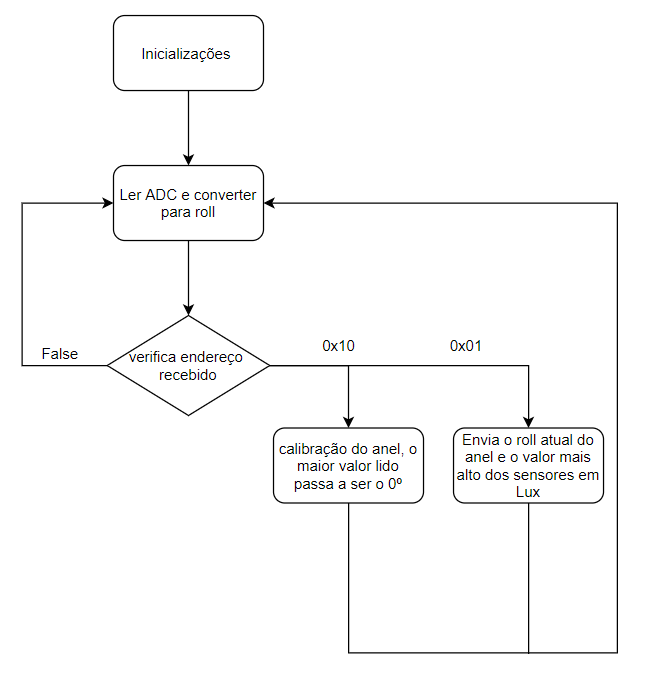
\includegraphics[scale=0.8]{Figuras/software.PNG}
\caption{Arquitectura de \textit{software} do anel}
\label{Rotulo}
\end{figure}